\section{Experiment Setup}

\subsection{Dataset}

The experiments are conducted on the Amazon Book Reviews dataset~\cite{ni2019justifying}, a large-scale e-commerce interaction log covering millions of user–item interactions across the book domain.
For evaluation, 100{,}000 users were sampled such that each user has at least one held-out test interaction.
The dataset statistics are summarised in Table~\ref{tab:dataset_stats}.

\begin{table}[H]
\centering
\caption{Dataset statistics used for evaluation.}
\label{tab:dataset_stats}
\begin{tabular}{lr}
\hline
\textbf{Statistic} & \textbf{Value} \\
\hline
Total evaluation users       & 100{,}000 \\
Test interactions per user   & 1 (leave-one-out) \\
Catalogue size (full)        & 3{,}080{,}829 items \\
Unique items in eval. sequences & 401{,}340 \\
Embedding cache size         & 575{,}288 items (2{,}356 MB) \\
Mean training sequence length & 378 interactions \\
Median training sequence length & 312 interactions \\
\hline
\end{tabular}
\end{table}

The training sequences are long-tailed: the 90th percentile exceeds 800 interactions while the 10th percentile has fewer than 50, reflecting a realistic mix of casual and power readers.
Figure~\ref{fig:dataset_statistics} visualises the distribution of training sequence lengths across all evaluation users.

\begin{figure}[H]
\centering
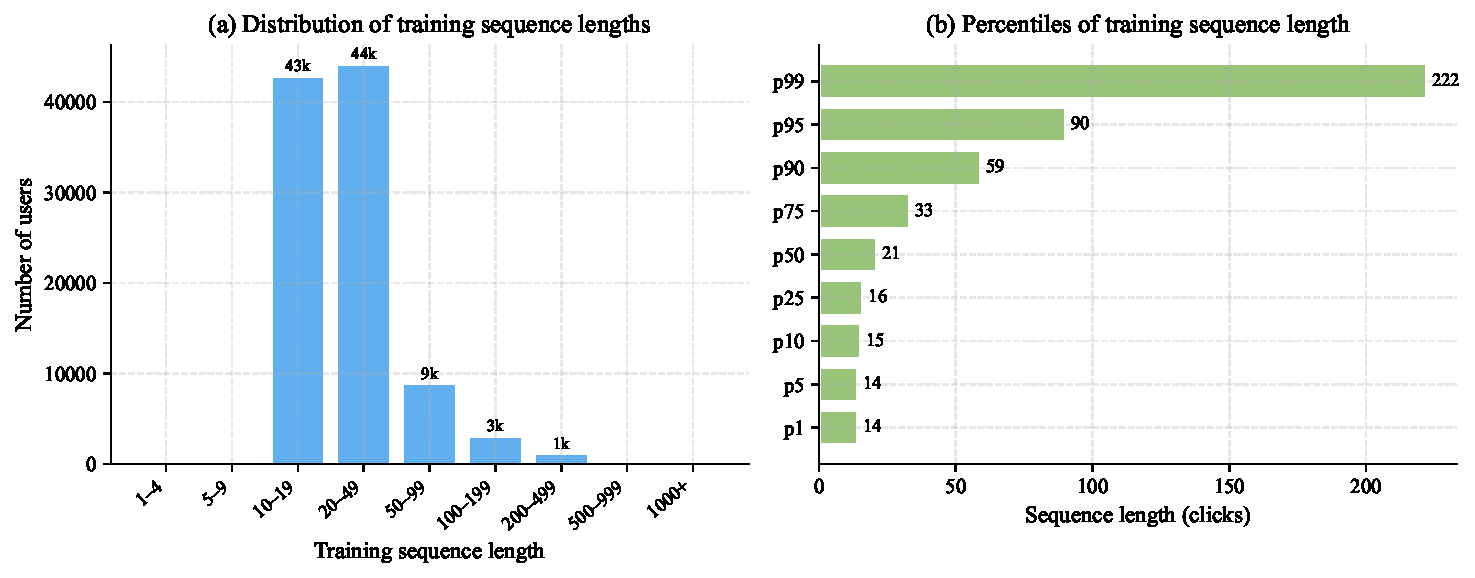
\includegraphics[width=\textwidth]{images/chapter5/fig_dataset_statistics}
\caption{Distribution of training sequence lengths across 100{,}000 evaluation users.
(a) Histogram by length bucket. (b) Percentiles showing that the median user has 312 interactions and the 90th-percentile user has over 800.}
\label{fig:dataset_statistics}
\end{figure}

\subsection{Evaluation Protocol}

A \textit{sampled negative} protocol is adopted, following the conventions of SASRec~\cite{kang2018self} and BERT4Rec~\cite{sun2019bert4rec}.
For each test user, the ground-truth item is ranked against $N$ uniformly sampled negative items that the user has not interacted with.
Two values of $N$ are considered:

\begin{itemize}
    \item $N = 99$ (primary): the standard academic setting used by most sequential recommendation benchmarks.
    Under this setting, a random baseline achieves HR@10 = 0.100 by chance.
    \item $N = 999$ (strict): a harder setting that approximates the full-catalogue difficulty.
    The random HR@10 drops to 0.010.
\end{itemize}

All primary results use $N = 99$.
Section~\ref{sec:end_to_end} reports both protocols for sensitivity analysis.
The evaluation seed is fixed to 42 for canonical runs; Section~\ref{sec:end_to_end} also reports multi-seed stability results.

\subsection{Metrics}

Three complementary retrieval metrics are reported at cut-off $k = 10$:

\begin{itemize}
    \item \textbf{HR@$k$} (Hit Rate): 1 if the ground-truth item appears in the top-$k$ ranked candidates, 0 otherwise. Averaged over all test users.
    \item \textbf{NDCG@$k$} (Normalised Discounted Cumulative Gain): position-sensitive ranking quality, rewarding earlier hits more strongly.
    \item \textbf{MRR@$k$} (Mean Reciprocal Rank): the reciprocal of the rank of the first relevant item, averaged across users.
\end{itemize}

HR@10 is the primary metric because it directly reflects whether a user would encounter a relevant recommendation in a top-10 list, which corresponds to the typical number of items displayed on a single screen.

\subsection{Baselines}

Five systems are compared to assess the contribution of each component:

\begin{enumerate}
    \item \textbf{Random Baseline}: uniform random ranking over the $N+1$ candidates. Provides a lower bound.
    \item \textbf{Content Baseline}: mean pooling of BGE-M3 embeddings over the user's training sequence, followed by cosine similarity ranking. Represents a simple semantic profile without sequential modelling.
    \item \textbf{GRU-SeqDQN}: a recurrent reinforcement-learning approach using a GRU-based policy network trained with Deep Q-Network objectives. Represents a prior sequential recommendation approach from the existing system.
    \item \textbf{DIF-SASRec (Pipeline B)}: the proposed Decoupled Intent-Feature Self-Attentive Recommendation model with separate content and category attention streams.
    \item \textbf{Pipeline A (Cleora + BGE-M3)}: behavioural co-purchase graph embeddings (Cleora) for candidate retrieval, re-ranked by BGE-M3 semantic similarity.
    \item \textbf{System ($A \cup B$)}: the combined output of Pipeline A and Pipeline B, taking the union of their top-10 sets with RRF-based re-ranking ($k = 60$).
\end{enumerate}

\subsection{Model Configurations}

Table~\ref{tab:model_config} summarises the key hyperparameters of the two proposed pipelines.

\begin{table}[H]
\centering
\caption{Model configuration for the proposed pipelines.}
\label{tab:model_config}
\begin{tabular}{p{5.2cm}p{7.8cm}}
\hline
\textbf{Parameter} & \textbf{Value} \\
\hline
\multicolumn{2}{l}{\textit{Pipeline B — DIF-SASRec}} \\
Architecture     & Decoupled Intent-Feature SASRec \\
Transformer blocks & 4 \\
Attention heads  & 8 \\
Hidden dimension & 512 \\
Max sequence length & 200 \\
Parameters       & $\approx$12.4M \\
Training users   & 100{,}000 (pretrained) \\
Epochs           & 30 \\
Batch size       & 2{,}048 \\
Optimizer        & AdamW with cosine LR annealing \\
Content veto $\tau$ & 0.3 (cosine threshold) \\
\hline
\multicolumn{2}{l}{\textit{Pipeline A — Cleora + BGE-M3}} \\
Graph embedding  & Cleora (co-purchase behavioral graph) \\
Cleora index size & 375{,}280 items \\
Profile encoder  & BGE-M3 (\texttt{BAAI/bge-m3}), 1{,}024-dim, fp16 \\
FAISS index (prod.) & HNSW, 1.7M vectors \\
FAISS index (eval.) & Flat exact, 3M vectors \\
RRF constant $k$ & 60 \\
\hline
\end{tabular}
\end{table}
